
\chapter{Choosing Between Alternatives}

Processing information is a linear activity. Listen to anyone describing
how something is performed and you will hear phrases like: 'first
get an X, turn it into a Y and feed it into the Z'. This is great
because mechanical processing of models is a linear activity too;
there is a close correspondence between real-world processes and their
modelled equivalent.

However, things are often not that simple. On closer inspection a
process can often be more like: 'select an X, find a way to turn it
into a Y and feed it into one of the Zs'. In this case processing
is not so obviously linear. What happens if the X that is selected
turns out to be the wrong choice when trying to make a Y? Can we go
back and try another X? If no Z is available who is at fault: the
X or the choice of Y?

The world is full of choices. Modelling the world often needs to take
account of choice. Once choice is admitted into a process, the \textit{scope}
of the choice becomes an important issue. How far can processing proceed
before a particular choice cannot be undone? In a linear activity,
undoing a choice within a particular scope is called \textit{backtracking,}
i.e. returning to the last choice point, selecting an alternative
and re-processing from that point.

Choice (or equivalently \textit{non-determinism}) is a property of
a model. Backtracking is a property of the execution engine for the
model. Backtracking is a way of implementing choice as a linear activity;
it is an important and often occurring pattern. This section is about
how to implement the pattern.


\section{A Choice Pattern}

Choice tends to occur as a pattern involving:

\begin{itemize}
\item A collection of elements to choose from (or alternative actions).
\item Something to do next with the selected element.
\item Something to backtrack with (a failure).
\end{itemize}
Each use of this pattern tends to be slightly different in the detail.
But the principle is generally the same. The pattern can be encoded
as follows:

\begin{lstlisting}
(1) @Operation select(S,next,fail)
(2)  if S->isEmpty
(3)  then fail()
     else
(4)  let e = S->sel then
(5)      S = s->excluding(e)
(6)  in next(x,@Operation() select(S,next,fail) end)
     end
   end
\end{lstlisting}The operation select (1) encodes the pattern. It takes 3 arguments:
S a set of elements to choose from, the activity to do next and a
fail for backtracking. The next activity is encoded as an operation
that is expecting an element and a fail. The fail argument is encoded
as an operation that takes no arguments and jumps to the last choice
point to choose an alternative.

The idea is that the next operation contains all future processing
for a selected element. Cruicially, the next operation may be invoked
more than once with different choices from S. Lines (4-6) show this
occurring, where an element e is selected from S and supplied to next.
The failure argument supplied to next is a new choice point; if it
is ever invoked then select is called again with fewer options to
choose from, \textit{but the same next and fail}. Therefore, select
can cause the same next argument to be invoked multiple times with
different elements chosen from S.

If select is ever invoked with no options (2) then the initial failure
argument is chosen. This allows chaining of different uses of select.

A slight variation on this pattern is the inclusion of a predicate
that controls whether the chosen element is valid or not:

\begin{lstlisting}
(1) @Operation select(S,next,pred,fail)
(2)  if S->isEmpty
(3)  then fail()
     else
(4)  let e = S->sel then
(5)      S = s->excluding(e)
(6)  in if pred(e)
(7)     then next(x,@Operation() select(S,next,pred,fail) end)
(8)     else select(S,next,pred,fail)
(9)     end
     end
   end
\end{lstlisting}The predicate is used in (6) to test the element. If pred is satisfied
then next is invoked as before (7), otherwise alternatives are tried
(8).

This pattern can be encoded as a language construct. The basic mechanism
involves repeated selection from a supplied set of alternatives. The
grammar below uses a locally defined recursive operation to continually
backtrack though the elements of a supplied set:

\begin{lstlisting}
@Grammar extends OCL::OCL.grammar
  Select ::= 
    '(' e = Name ',' f = Name ')' 'from' s = Exp 
        test = ('when' Exp | [| true |]) 'do' 
        body = Exp 
    'else' fail = Exp 'end' 
  { [|
      @Letrec
        select = 
          @Operation(S,<f>)
            if S->isEmpty
            then <Var(f)>()
            else 
              let <e> = S->sel then
                  S = S->excluding(<Var(e)>) then
                  <f> = @Operation() select(S,<Var(f)>) end
              in if <test>
                 then <body>
                 else <f>()
                 end
              end
            end
          end
       in select(<s>,@Operation() <fail> end)
       end
     |] }.
end
\end{lstlisting}Instead of defining a selection operation each time choice is used,
the selection construct can be used as follows:

\begin{lstlisting}
@Select(e,f) from S do
  next(e,f)
else fail()
end
\end{lstlisting}The variable e is initially bound to an element selected from the
set S and the body of the construct (after the do) is performed. The
variable f is bound to an operation; is f is ever invoked (with 0
args) then another element of S is selected and the body is performed
again. Subsequent uses of f have the same effect until S is exhausted
at which point the alternative part of the construct (after the else)
is performed.

%
\begin{figure}
\begin{center}

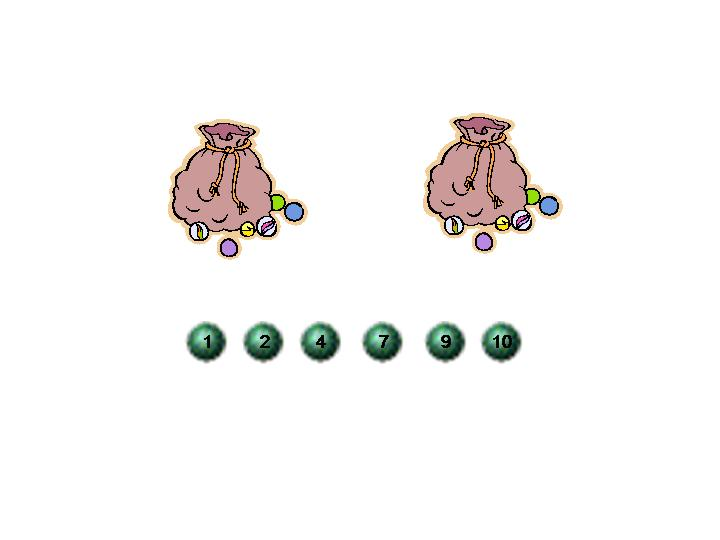
\includegraphics[width=12cm]{LanguageEngineering/Choice/Images/Sacks}

\caption{\label{fig:Two-sacks-with}Two sacks with numbered balls}

\end{center}
\end{figure}


Consider a situation, shown in figure \ref{fig:Two-sacks-with} where
two sacks contain an arbitrary collection of numbered balls. Balls
are selected from each sack in turn and placed in a line. The idea
is to wind up with a sequence of balls whose numbers form an ascending
sequence.

Since it is not permitted to look inside the sacks when selecting
a ball, things can go wrong at some point during the process; although
it is always possible to select the balls in a way that achieves the
desired outcome. If things go wrong then balls can be put back (balls
are appropriately marked as to which sack they came from), and the
selection restarted from any point.

The sacks can be modelled as follows:

\begin{lstlisting}
@Class Sack
  @Attribute balls : Set(Integer) end
  @Attribute other : Sack (!,?) end
  @Constructor(balls) ! end
end
\end{lstlisting}where two sacks are set up as follows:

\begin{lstlisting}
let s1 = Sack(Set{1,7,3,5,9});
    s2 = Sack(Set{8,2,6,4,10})
in s1.setOther(s2);
   s2.setOther(s1)
end
\end{lstlisting}The process of selection is to be modelled as an operation on Sack
that builds a sequence of integers (balls) by ping-ponging between
the receiver and 'other', each optionally adding an integer. What
happens when there are balls left to choose, but which cannot be added
to the sequence because their numbers are too low? Is it always possible
to select so that this situation does not occur? Inspection of the
rules shows that this is not the case (the contents of the other sack
cannot be inspected). Therefore, a stalemate situation can occur,
therefore backtracking is a candidate modelling technique.

The rest of this section builds up the implementation of an operation
defined by Sack for ordering the elements selected from two sacks.
The operation is called with no arguments:

\begin{lstlisting}
@Operation order()
(1)  self.order(Seq{},
(2)    @Operation(orderedBalls,next,fail) 
(3)      other.order(orderedBalls, 
(4)        @Operation(orderedBalls,next2,fail) 
(5)          next(orderedBalls,next2,fail) 
(6)        end,fail) 
       end,
(7)    @Operation() 
         "Error!" 
       end)
end
\end{lstlisting}The ordering operation needs to initialise the ordered balls and create
an initial next and fail. Line (1) calls a second Sack operation called
order that has these as arguments. The initial collection of ordered
balls is Seq\{\} (1), the initial next operation and fail are supplied
in lines (2) and (7).

In this example, each next takes 3 arguments: the current sequence
of ordered balls, a next for the other sack and a fail. At line (2)
the initial next calls the ordering operation for the other sack (3)
passing it a next at (4) that ping-pongs back.

The initial fail (7) returns an error value because it should always
be possible to order the balls, i.e. this should never occur.

The second order operation is defined as follows:

\begin{lstlisting}
@Operation order(orderedBalls,next,fail)
(1)  if not other.allChosen(orderedBalls)
     then 
(2)    self.order(orderedBalls,balls,next,
(3)      @Operation() 
           next(orderedBalls,
(4)          @Operation(orderedBalls,next,fail) 
(5)            self.order(orderedBalls,next,fail) 
             end,fail) 
         end)
(6)  else self.order(orderedBalls,balls,next,fail)
     end
end
\end{lstlisting}If the other sack is empty (1) then the selection continues with the
current sack (7). If the other sack is not empty then there is a choice:
add an element from the current sack (2) and continue or just continue.
This alternative is encoded by extending the fail (3) so that if things
go wrong, the curren sack is skipped. If it is skipped then play resumes
with the current sack due to the next continuation (4-5).

The final operation uses Select to continually select from the available
balls:

\begin{lstlisting}
@Operation order(orderedBalls,balls,next,fail)
  if balls->isEmpty
  then orderedBalls
  else
    @Select(ball,f) from balls 
      when not orderedBalls->exists(b | b > ball) do
        next(orderedBalls + Seq{ball},
          @Operation(orderedBalls,next,fail) 
            let balls = balls->excluding(ball)
            in self.order(orderedBalls,balls,next,fail)
            end
          end,f)
    else fail()
    end
  end
end
\end{lstlisting}
\section{Finding a Route}

%
\begin{figure}
\begin{center}

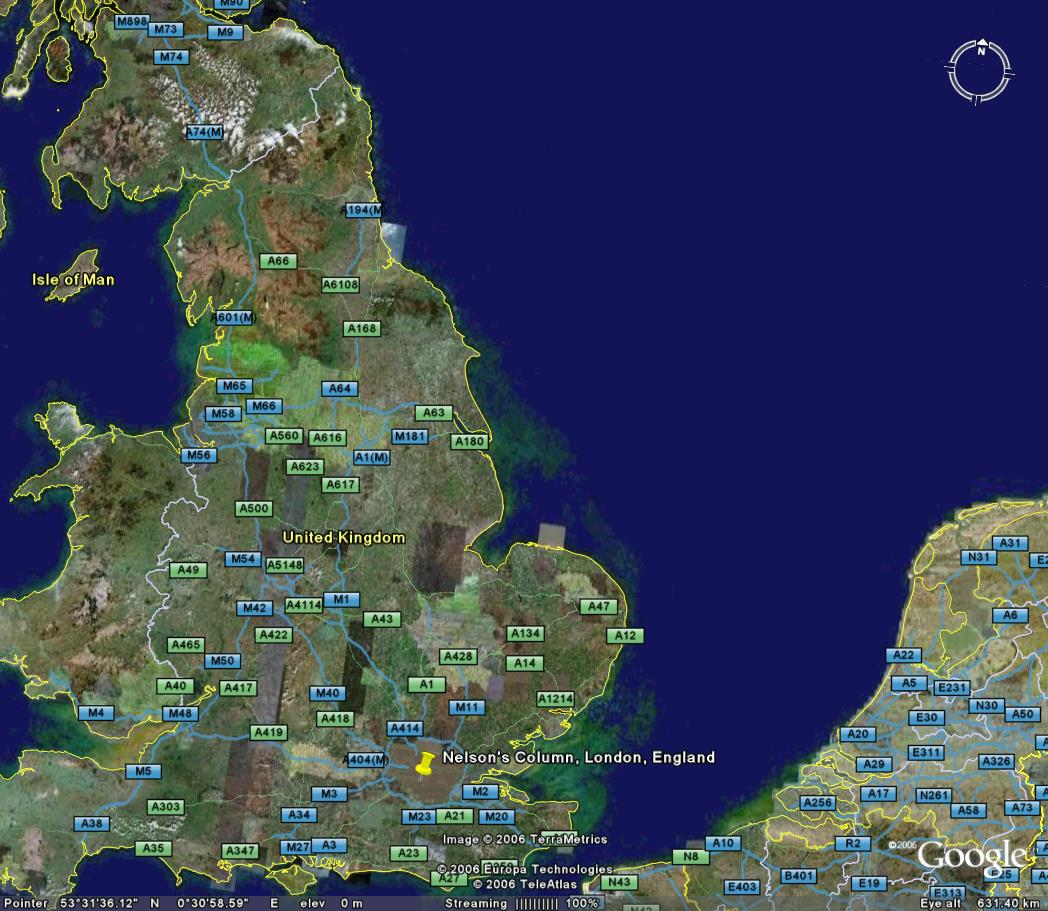
\includegraphics[width=12cm]{LanguageEngineering/Choice/Images/UK}

\caption{\label{fig:Routes-in-the}Routes in the UK}

\end{center}
\end{figure}


Figure \ref{fig:Routes-in-the} shows a map of the UK with locations
and roads. One way of modelling this information is using the graph
construct defined in section \ref{sub:Graphs}:

\begin{lstlisting}
@Graph(Routes,City,Road)
    Birmingham()
    Brighton()
    Bristol()
      A48 -> Swansea
    Carlisle()
      A74 -> Glasgow
      A69 -> Newcastle
    Glasgow()
      M8 -> Edinburgh
      M80 -> Perth
    London()
      M23 -> Brighton
      A12 -> Ipswich
      A41 -> Oxford
      A3 -> Portsmouth
      M4 -> Bristol
      M1()->Leeds
      A1()->Peterborough
      M11()->Cambridge
    Hull()
    Ipswich()
    Leeds()
      M62()->Bradford
      M62 -> Hull
      A1()->Newcastle
    Oxford()
      M40 -> Birmingham
    Perth()
      M90 -> Edinburgh
    Portsmouth()
    Swansea()
    Bradford()
      M62()->Manchester
    Newcastle()
      A1()->Edinburgh
    Manchester()
      M61 -> Preston
    Preston()
      M6 -> Carlisle
    Peterborough()
      a1 -> Newcastle
    Cambridge()
    Edinburgh() 
      A91()-> Dundee
    Dundee()
      A956()->Aberdeen
    Aberdeen()
end
\end{lstlisting}Each node of the graph is a city. Each edge of the graph is a road
labelled with its name. For example from London it is possible to
go to Brighton using the M23 (and vice versa), and possible to go
to Bristol using the M4.

Consider how to find a route from one city to another. Suppose you
want to get from London to Carlisle. It is possible via the M1, A1
and then A69. Alternatively, you could go A1, A1, A69. In principle
there are many routes between two cities. Ignoring distance and other
criteria that might lead to selecting one route over another, the
only rule that should be applied is that a route does not pass through
the same city twice.

How might the construction of a route be modelled? Given a start and
end city, if there is a road linking the two then a route is found.
Otherwise, any road from the start (or end) can be selected leading
to a new start (or end) point. Given the new start (or end) then the
process can be repeated until it can be shown that no route exists
(remember you cannot go through the same city twice) or a route is
found. Given that choices are made, if no route can be found then
backtracking can b employed to return and make an alternative choice.

The class Routes extends Graph with an operation for finding a route:

\begin{lstlisting}
(1) @Operation route(source:String,target:String)
(2)   self.route(Set{},source,target,
(3)     @Operation(usedRoads,path,fail) 
(4)       path 
        end,
(5)     @Operation() 
         "NONE" 
       end)
   end
\end{lstlisting}Given the names of the source and target cities (1), a route is consructed
by calling another operation with a set of used roads, the source,
target, a next (3) and a fail (5). The initial fail is invoked when
no route exists, it returns the special no-route-available value NONE.

A next expects a set of used roads, a path and a fail. The path links
the source and target cities and is a sequence of road names.

The second route operation is defined below:

\begin{lstlisting}
@Operation path(usedRoads,source,target,next,fail)
 if source = target
 then succ(usedRoads,Seq{},fail)
 else
  @Select(road,otherRoad) 
   from self.edgesIncidentOn(source) - usedRoads do 
    self.pathAfter(
     usedRoads,source,target,road,otherRoad,next,fail)
   else 
    @Select(road,otherRoad) 
     from self.edgesIncidentOn(target) - usedRoads do
      self.pathBefore(
       usedRoads,source,target,road,otherRoad,next,fail)
     else fail()
    end
  end
 end
end
\end{lstlisting}\begin{lstlisting}
@Operation pathAfter(usedRoads,source,target,road,otherRoad,succ,fail)
       self.path(usedRoads->including(road),road.otherEnd(source),target,
         @Operation(usedRoads,path,fail)
           succ(usedRoads,Seq{road.label()} + path,fail)
         end,
         otherRoad)
     end
@Operation pathBefore(usedRoads,source,target,road,otherRoad,succ,fail)
       self.path(usedRoads->including(road),source,road.otherEnd(target),
         @Operation(usedRoads,path,fail)
           succ(usedRoads,path + Seq{road.label()},fail)
         end,
         otherRoad)
     end
\end{lstlisting}
\section{Explanation and NoGood Sets}

Patterns of search (as described above) can be encoded using language
constructs. Typically these involve success and failure continuations
that maintain the state of the search and provide a convenient mechanism
for branching. Continuations make it easy to backtrack when it is
found that an incorrect branch has been selected. These techniques
work well for finding a configuration amongst a number of alternatives
such that the configuration satisfies a given condition. However,
extra work is required to explain the lack of a satisfactory configuration. 

One technique is to invert the condition that selects a correct configuration
and to use it to explain why no satisfactory configuration could be
found. Instead of selecting a single satisfactory configuration, such
an inversion produces a collection of configurations, each of which
has a problem. Such configurations are sometimes referred to as \emph{noGood}
sets. This section describes an application that uses search to select
a configuration of business components; noGood sets are used to explain
why a solution cannot be found.

Consider developing a business plan. The business must set out its
\emph{goals} in terms of what the business wants to achieve. Each
goal is supported by a collection of \emph{tactics} each of which
describes an activity or approach that claims to achieve the goal.
In addition, a goal may be decomposed into a collection of child goals;
achieving all the child goals individually is the same as achieving
the overall goal. In order to implement a given tactic it is necessary
to allocate some resource. Resource is provided by organizational
\emph{units}, which may be company departments or individuals.

A goal may be \emph{achieved} if it has a supporting tactic that is
adequately resourced; or may be achieved if all of its children are
achieved by the same rule. It is important that a company does not
over-commit its resources, therefore a goal can only be achieved if
the unit resource limits are not exceeded.

Here is a high-level goal for a telephone banking business:

\begin{center}
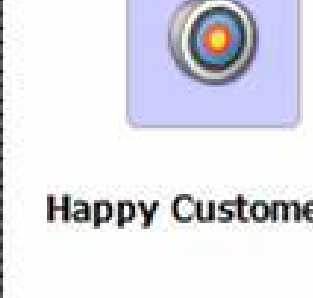
\includegraphics[width=5cm]{LanguageEngineering/Choice/Images/Goal}
\end{center}

The business will
be successful if it has happy customers. This goal can be decomposed
into any number of sub-goals:

\begin{center}
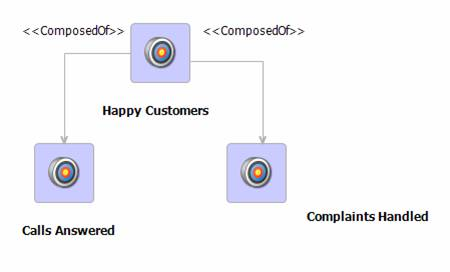
\includegraphics[width=5cm]{LanguageEngineering/Choice/Images/SubGoals}
\end{center}

where
a customer is happy if their calls are answered effectively and their
complaints are handled. Each of the sub-goals has any number of tactics
that will achieve the goal:

\begin{center}
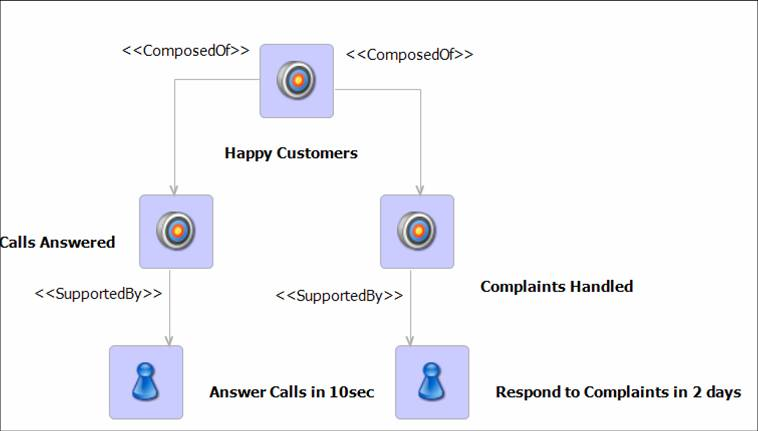
\includegraphics[width=5cm]{LanguageEngineering/Choice/Images/Tactics}
\end{center}

Finally, the tactics need to be resourced by an organization unit.
A unit may resource more than one tactic and a tactic may be resourced
by more than one unit. In this case the unit is a telephone call centre:

\begin{center}
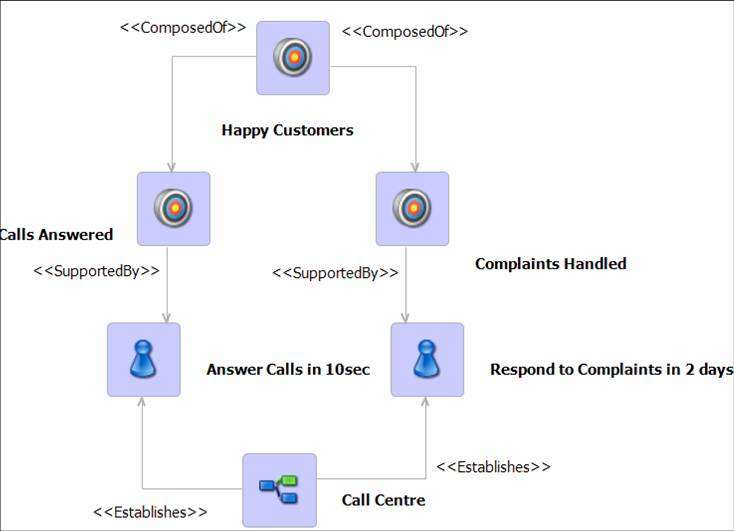
\includegraphics[width=5cm]{LanguageEngineering/Choice/Images/Units}
\end{center}


The models shown above can be used as part of a business as a decision
support solution. Each model describes the goals the business intends
to achieve and how the goals are to be implemented and resourced.
The solution provides feedback in terms of the options for resourcing
the tactics that achieve the goals. If the goals cannot be achieved
then the solution will provide feedback on why the different resourcing
options fail.

The rest of this section is in two parts: the first part describes
how an engine is defined that finds a resourcing solution; the second
part describes how noGood sets are used to provide feedback when there
is no solution.

%
\begin{figure}
\begin{center}

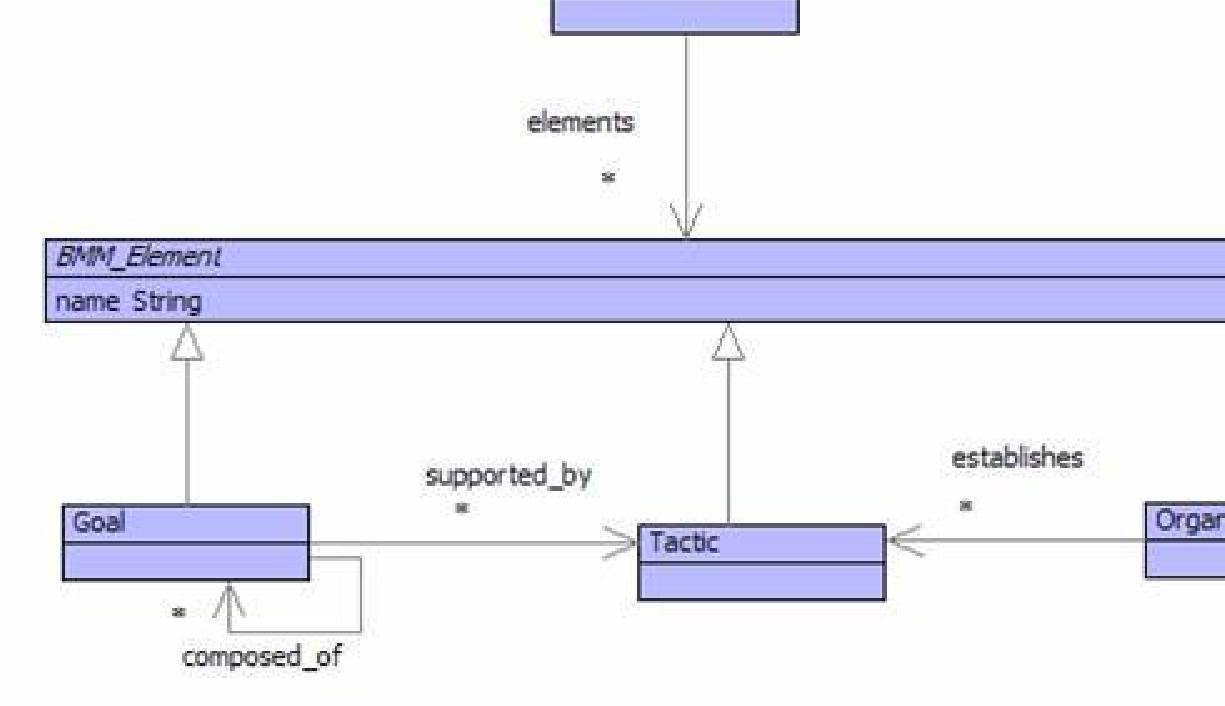
\includegraphics[width=12cm]{LanguageEngineering/Choice/Images/BMMModel}

\caption{The Business Motivation Model \label{fig:The-Business-Motivation}}

\end{center}
\end{figure}


%
\begin{figure}
\begin{center}

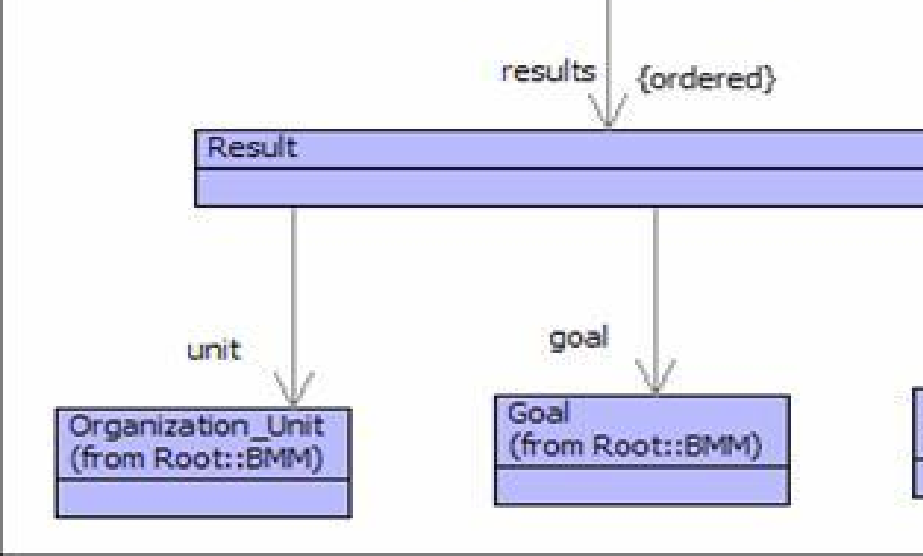
\includegraphics[width=12cm]{LanguageEngineering/Choice/Images/Results}

\caption{Configuration Results\label{fig:Configuration-Results}}

\end{center}
\end{figure}


Figure \ref{fig:The-Business-Motivation} shows a model of the business
concepts used by the solution. Figure \ref{fig:Configuration-Results}
shows a report model that is produced when there is a solution consisting
of a collection of results each of which associates a goal, a tactic
and an organization unit.

The following rules are applied to find a solution. A goal g is achievable
when:

\begin{enumerate}
\item g is supported by at least one tactic that is established by at least
one organization unit; or
\item g has at least one sub-goal and each sub-goal is achieved; and
\item the number of tactics supported by each unit does not exceed the resource
for the unit.
\end{enumerate}
The rules are implemented as an operation called achievable that is
defined below. The arguments of the operation form the context for
the achievable-engine. It is supplied with a goal, a table of resources,
the current results and continuations for success and failure. The
table of resources is an a-list mapping unit names to the current
amount of resource available for that unit. The results are just a
collection of result instances. 

\begin{lstlisting}
context BMM_Model
  @Operation achievable(goal,resources,results,succ,fail)
    @Select tactic:Tactic from goal.getSupported_by() do
      @Select unit:Organization_Unit from self.getElements() 
        when unit.establishes(tactic)
        do @Result(goal,tactic,unit) 
             @Use(unit) end
           end
      end
    else
      @Unless goal.getComposed_of().isEmpty() do 
        @ForAll child in goal.getComposed_of() do
          self.achievable(child,resources,results,succ,fail)
        end
      end
    end
  end
\end{lstlisting}The success and fail continuations are used to implement a backtracking
mechanism. The rules are implemented by the achievable-engine in terms
of search. A choice-point arises when there is more than one tactic
that could be chosen to support a goal and when there is more than
one unit that could be chosen to establish a tactic. In both cases,
one of the options is chosen and a choice point is created that will
be used if ever the search fails. 

Failure occurs when a goal cannot be achieved because it has no tactics
or a tactic has no establishing unit. The resource associated with
a unit is reduced by 1 each time the unit is used to establish a tactic.
Once the count reaches 0 the unit cannot be used again; a subsequent
attempt to select the unit causes backtracking.

The achievable-engine uses language constructs that are specifically
designed to support the business solution. These constructs are: Select
which is used to select from a collection; Result which is used to
produce a result; Use which is used to reduce the amount of available
resource for a unit; Unless which is used to place a guard on an action;
and, ForAll which is used to require a condition holds for all element
of a collection. These language constructs use the arguments of the
engine as 'globals' and are implemented as follows.

The language construct for Select uses the selection operation to
try each element of a collection:

\begin{lstlisting}
context Root
  @Class Select extends Sugar
    @Attribute var        : String end
    @Attribute type       : Performable end
    @Attribute collection : Performable end
    @Attribute body       : Performable end
    @Attribute guard      : Performable end
    @Attribute alt        : Performable end
    @Constructor(var,type,collection,guard,body,alt) ! end
    @Grammar extends OCL::OCL.grammar
      Select ::= 
        v = Name ':' t = Exp 'from' c = Exp g = Guard 'do' 
          b = Exp a = Alt 'end' {
            Select(v,t,c,g,b,a)
      }.
      Guard ::=
        'when' Exp
      | { [| true |] }.
      Alt ::= 
        'else' Exp
      | { [| fail() |] }.
    end
  end
\end{lstlisting}The desugar operation for Select builds up a choice-point through
the fail continuations:

\begin{lstlisting}
context Select
  @Operation desugar() 
    [| let // Filter on the type of the elements...
           C = <collection>.asSeq()->select(x | 
             x.isKindOf(<type>)) then
           // Filter using the guard...
           C = C->select(<var> | <guard>) then
           // Set up the action to perform...
           action = 
             @Operation(<var>,fail) 
               <body> 
             end then
           // The final fail performs the alternative action...
           finalFail = 
             @Operation() 
               <alt> 
             end then
           // Build up the choice-tree using fails...
           fail = C->iterate(x fail = finalFail | 
                    @Operation() 
                      action(x,fail) 
                    end)
       in // Perform the first choice...
          fail()
       end |]
  end
\end{lstlisting}The Result construct adds a new result to the current collection of
results. This establishes a new collection of results for the scope
of the Result body:

\begin{lstlisting}
@Class Result extends Sugar
    @Attribute goal   : Performable end
    @Attribute tactic : Performable end
    @Attribute unit   : Performable end
    @Attribute body   : Performable end
    @Constructor(goal,tactic,unit,body) ! end
    @Grammar extends OCL::OCL.grammar
      Result ::= '(' g = Exp ',' t = Exp ',' u = Exp ')' 
        b = Exp 'end' {
          Root::Result(g,t,u,b)
      }.
    end
    @Operation desugar()
      [| let result = Result(<goal>,<tactic>,<unit>) then
             results = results->including(result)
         in <body>
         end
      |]
    end
  end
\end{lstlisting}When a unit is used to establish a tactic, the number of resources
associated with the unit must be reduced by one. However a unit cannot
use more resource than it owns, therefore if the resources are exhausted
for the required unit then engine uses fail to select an alternative:

\begin{lstlisting}
@Class Use extends Sugar
    @Attribute unit : Performable end
    @Attribute body : Performable end
    @Constructor(unit,body) ! end
    @Grammar extends OCL::OCL.grammar
      Use ::= '(' u = Exp ')' b = Body 'end' {
        Use(u,b)
      }.
      Body ::=
        Exp
      | { [| succ(resources,results,fail) |] }.
    end
    @Operation desugar()
      [| let name = <unit>.getName() then
             resource = resources.lookup(name)
         in if resource = 0
            then fail()
            else 
              let resources = resources.bind(name,resource - 1)
              in <body>
              end
            end
         end |]
    end
  end
\end{lstlisting}The Unless construct simply places a guard on an action; if the guard
fails then an alternative is found using the fail continuation:

\begin{lstlisting}
@Class Unless extends Sugar
    @Attribute guard : Performable end
    @Attribute body : Performable end
    @Constructor(guard,body) ! end
    @Grammar extends OCL::OCL.grammar
      Unless ::= g = Exp 'do' b = Exp 'end' {
        Unless(g,b)
      }.
    end
    @Operation desugar()
      [| if <guard>
         then fail()
         else <body>
         end
      |]
    end
  end
\end{lstlisting}The ForAll construct requires a condition to hold for all elements
of a collection. This is achieved using the success continuation;
each element of the collection is selected and the success continuation
returns to the collection to try the next element:

\begin{lstlisting}
@Class ForAll extends Sugar
    @Attribute var        : String end
    @Attribute collection : Performable end
    @Attribute body       : Performable end
    @Constructor(var,collection,body) ! end
    @Grammar extends OCL::OCL.grammar
      ForAll ::= v = Name 'in' c = Exp 'do' b = Exp 'end' {
        ForAll(v,c,b)
      }.
    end
    @Operation desugar()
      [| let next = 
               @Operation(<var>,resources,results,succ,fail) 
                 <body> 
               end
         in <collection> ->iterate(x succ = succ |
              @Operation(resources,results,fail)
                next(x,resources,results,succ,fail)
              end )
         end |]
    end
  end
\end{lstlisting}That concludes the language constructs for the achievable-engine.
The search is controlled using continuations so that all possible
combinations of goal, tactic and unit are tried to see if they are
compatible. When an illegal combination is encountered, the fail continuation
is used to backtrack. Therefore, the engine will find a suitable collection
of results if they exist. 

When no suitable combination of business elements exists, the engine
returns no value. It simply reports that the goal cannot be achieved.
The rest of this section describes how a noGood sets can be constructed
to explain the reasons why a solution cannot be found.

A noGood set is a combination of goals, tactics and units that invalidates
the achievable rules defined earlier. The rules are invalidated when
a goal has no tactics, when all tactics for a goal lack suitable organization
units, or when all the sub-goals of a goal invalidate the rules. When
no valid solution can be found for a goal, it is safe to assume that
at least one noGood set exists for the goal; there may bemore than
one noGood set and it is useful to report all of them.

The following operation constructs the noGood sets for a goal:

\begin{lstlisting}
context BMM_Model
  @Operation noGoods(goal)
    self.noTacticsOrChildren(goal) +
    self.noEstablishingUnits(goal) +
    self.overusedUnits(goal) +
    self.failingChildren(goal)
  end
\end{lstlisting}There are four reasons for a noGood set. Each reason is implemented
as a separate operation. The first operation constructs a singleton
set Unachievable(g) when the goal g has no tactics and no children:

\begin{lstlisting}
context BMM_Model
  @Operation noTacticsOrChildren(goal)
    @Cmp [Set] Set{Unachievable(goal)} where
      ? goal.noChildren() and 
        goal.noTactics() 
    end
  end
\end{lstlisting}If a goal has a tactic with no establishing units then a noGood set
contains Unestablished(g,t):

\begin{lstlisting}
context BMM_Model
  @Operation noEstablishingUnits(goal)
    @Cmp [Set] Set{Unestablished(goal,tactic)} where
      tactic <- goal.tactics(), 
      ? self.noEstablishingUnit(tactic)
    end 
\end{lstlisting}If a goal has a tactic with a unit then, since we know that there
are no good sets, the unit must be overused (or the noGood set is
incomplete). The following operation records allocations that will
become illegal when combined with other elements:

\begin{lstlisting}
contxt BMM_Model
  @Operation overusedUnits(goal)
    @Cmp [Set] Set{Allocation(goal,tactic,unit)} where
      tactic <- goal.tactics(), 
      unit <- self.establishingUnits(tactic)
    end
\end{lstlisting}Finally, each of the children of a goal must fail in a noGood set.
The following operation calculates the noGood sets for each child
and then combines them:

\begin{lstlisting}
context BMM_Model
  @Operation failingChildren(goal)    
    @Iterate1 child <- goal.children() 
      initially NG = Set{Set{}} do
        @Cmp [Set] options1 + options2 where
          options1 <- self.noGoods(child),
          options2 <- NG
        end
      else Set{}
    end
  end
\end{lstlisting}Finaly, each noGood set must be interpreted to produce an explanation
of why a good set could not be produced. The following operation translates
the noGood sets into strings that explain why each fails:

\begin{lstlisting}
context BMM_Model
  @Operation noGoodDisplays(NGs)
    @Cmp [Set] u.goal.getName() + " has no tactics or children." where 
       NG <- NGs,
       u:Unachievable <- NG
     end +
     @Cmp [Set] u.goal.getName() + 
            " cannot be established by " + 
            u.tactic.getName() + 
            " because it has no supporting units." where 
       NG <- NGs,
       u:Unestablished <- NG 
     end +
     @Cmp [Set] o.getName() + " is overused." where 
       NG <- NGs,
       o:Organization_Unit <- self.getElements().asSeq(), 
       ? @Cmp a where 
           a:Allocation <- NG, 
           ? a.unit = o
         end->size > self.resources().lookup(o.getName()) 
     end
   end
\end{lstlisting}